\subsection{Generating intelligent icons}
Let $z_{C_{\kappa},.}$ be the vector of normalized importance values within cluster $C_\kappa$ for all motifs. As noted earlier, because our analysis was limited to length two motifs, the total number of motifs is $\beta^2$. Therefore $z_{C_{\kappa},.}$ can be reshaped to a square icon with side lengths $\beta$. The function named reshape() - implemented in either Matlab or Numpy - was used with $z_{C_{\kappa},.}$ and the number of columns and rows as parameters to generate icon matrices. Reshape() in Matlab orders differently than in Numpy, but specifying to use Fortran order in Numpy recreates Matlab behavior. However, since our analysis was done in Numpy, for the sake of convenience Numpy's default behavior was used, which lays motifs out along the icon as shown in figure \ref{fig:example_icon}. Pixel colors correspond to $z_{C_{\kappa},m}$ values and are capped at $[-3,3]$, corresponding to $-3$ and $+3$ standard deviations from the mean.

\begin{figure}[h]
  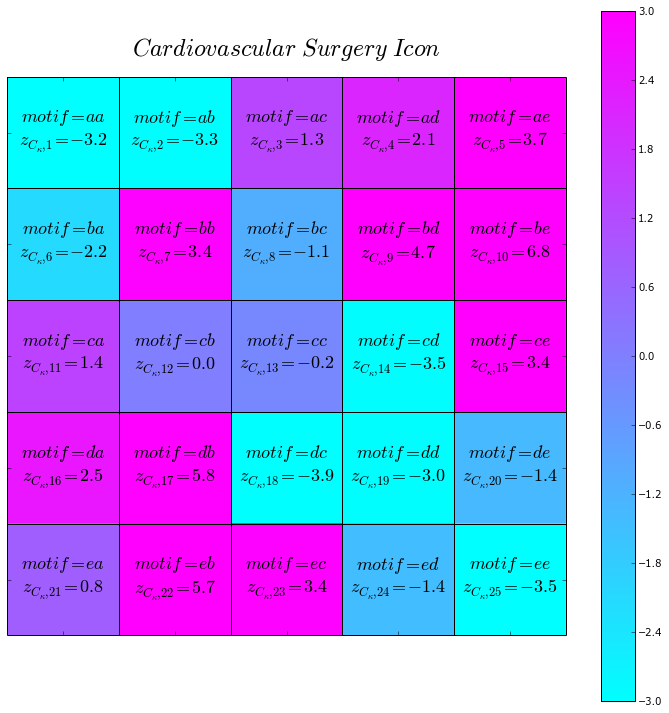
\includegraphics[scale=0.35]{./Figures/example_icon.png}\\
  \caption{Sample icon for the cluster of patients that underwent cardiovascular surgery, with text overlaying each pixel describing how the color was calculated. \textbf{Needed: redo this once decision is made on normalized/unnormalized SAX}}\label{fig:example_icon}
\end{figure} 